% CVPR 2027 Paper Template; see https://github.com/cvpr-org/author-kit

\documentclass[10pt,twocolumn,letterpaper]{article}

%%%%%%%%% PAPER TYPE  - PLEASE UPDATE FOR FINAL VERSION
% \usepackage{cvpr}              % To produce the CAMERA-READY version
\usepackage[review]{cvpr}      % To produce the REVIEW version
% \usepackage[pagenumbers]{cvpr} % To force page numbers, e.g. for an arXiv version

% Import additional packages in the preamble file, before hyperref
%% This file contains a number of tweaks that are typically applied to the main document.
%% They are not enabled by default, but can be enabled by uncommenting the relevant lines.


%%
%% Official support for 2-column teaser figure
%%
\usepackage{cuted} %< for strip environment

%%
%% For auto-referencing of figures (see fig/teaser.tex and \label{} therein) 
%%
\usepackage{currfile} %< for \currfilebase macro

%%
%% caption and (global) spacing overrides
%%
\usepackage{caption} %< for "\captionof" commands (teaser)
% \setlength{\abovecaptionskip}{.5em} % space above caption
% \setlength{\belowcaptionskip}{1em} % space below caption

%%
%% Inline annotations; for predefined colors, refer to "dvipsnames" in the xcolor package:
%% https://tinyurl.com/overleaf-colors
%%
\newcommand{\red}[1]{{\color{red}#1}}
\newcommand{\todo}[1]{{\color{red}#1}}
\newcommand{\TODO}[1]{\textbf{\color{red}[TODO: #1]}}
%%
%% Disable for camera ready / submission by uncommenting these lines:
%%
% \renewcommand{\TODO}[1]{}
% \renewcommand{\todo}[1]{#1}

%%
%% Pointers into the supplement.  The supplement is a separate file (due 11-23), so the main text cannot
%% \cref into it.  \supp{label} prints "the supplement"; with \withsupptrue (flip it below, only for a draft
%% that compiles sec/X_suppl in) it also prints the section, so that every pointer can be checked.
%%
\newif\ifwithsupp
\withsuppfalse
\newcommand{\supp}[1]{the supplement\ifwithsupp~(\cref{#1})\fi}

%%
%% Work harder in optimizing text layout. Typically shrinks text by 1/6 of page, enable
%% it at the very end of the writing process, when you are just above the page limit.
%%
% \usepackage{microtype}

%%
%% Heading gaps, rigid (no plus/minus): sections 1.5 × the template default; paragraphs 3.11ex (1.5 × less 25%, less 15%; user 11-16).
%% 3.11ex is 0.96 × the article default's natural size and inside its own shrink range (3.25ex minus .2ex = 3.05ex): do NOT go below 3.05ex.
%%   \section   cvpr.sty: -10pt / 7pt     → -15pt / 10.5pt
%%   \paragraph article:  3.25ex plus 1ex minus .2ex → 3.11ex fixed
%% \parskip kept at 0pt so twocolumn \flushbottom cannot re-stretch gaps apart.
%% Run-in/@startsection kept; do not edit cvpr.sty (RED_FILE §1.3).
%%
\setlength{\parskip}{0pt}
\makeatletter
\def\cvprsection{\@startsection {section}{1}{\z@}%
  {-15pt}{10.5pt} {\large\bf}}
\renewcommand{\paragraph}{\@startsection{paragraph}{4}{\z@}%
  {3.11ex}%
  {-1em}%
  {\normalfont\normalsize\bfseries}}
\makeatother

%%
%% Globally adjusts space between figure and caption.
%%
% \setlength{\abovecaptionskip}{.5em}

%%
%% Allows "the use of \paper to refer to the project name"
%% with automatic management of space at the end of the word.
%%
% \usepackage{xspace}
% \newcommand{\paper}{ProjectName\xspace}

%%
%% Commonly used math definitions.
%%
% \DeclareMathOperator*{\argmin}{arg\,min}
% \DeclareMathOperator*{\argmax}{arg\,max}

%%
%% Tighten underline.
%%
% \usepackage{soul}
% \setuldepth{foobar}


\definecolor{cvprblue}{rgb}{0.21,0.49,0.74}
\usepackage[pagebackref,breaklinks,colorlinks,allcolors=cvprblue]{hyperref}

\def\confName{CVPR}
\def\confYear{2027}

%%%%%%%%% TITLE
\title{Seshat-Star: Unambiguous, Rich, and Verifiable Spatial Cues in Natural Language Make 3D Models Sharper in Space}

%%%%%%%%% AUTHORS (hidden in review mode)
\author{Anonymous CVPR submission\\
Paper ID \TODO{xxxx}
}

\begin{document}
\maketitle
\begin{strip}
\centering
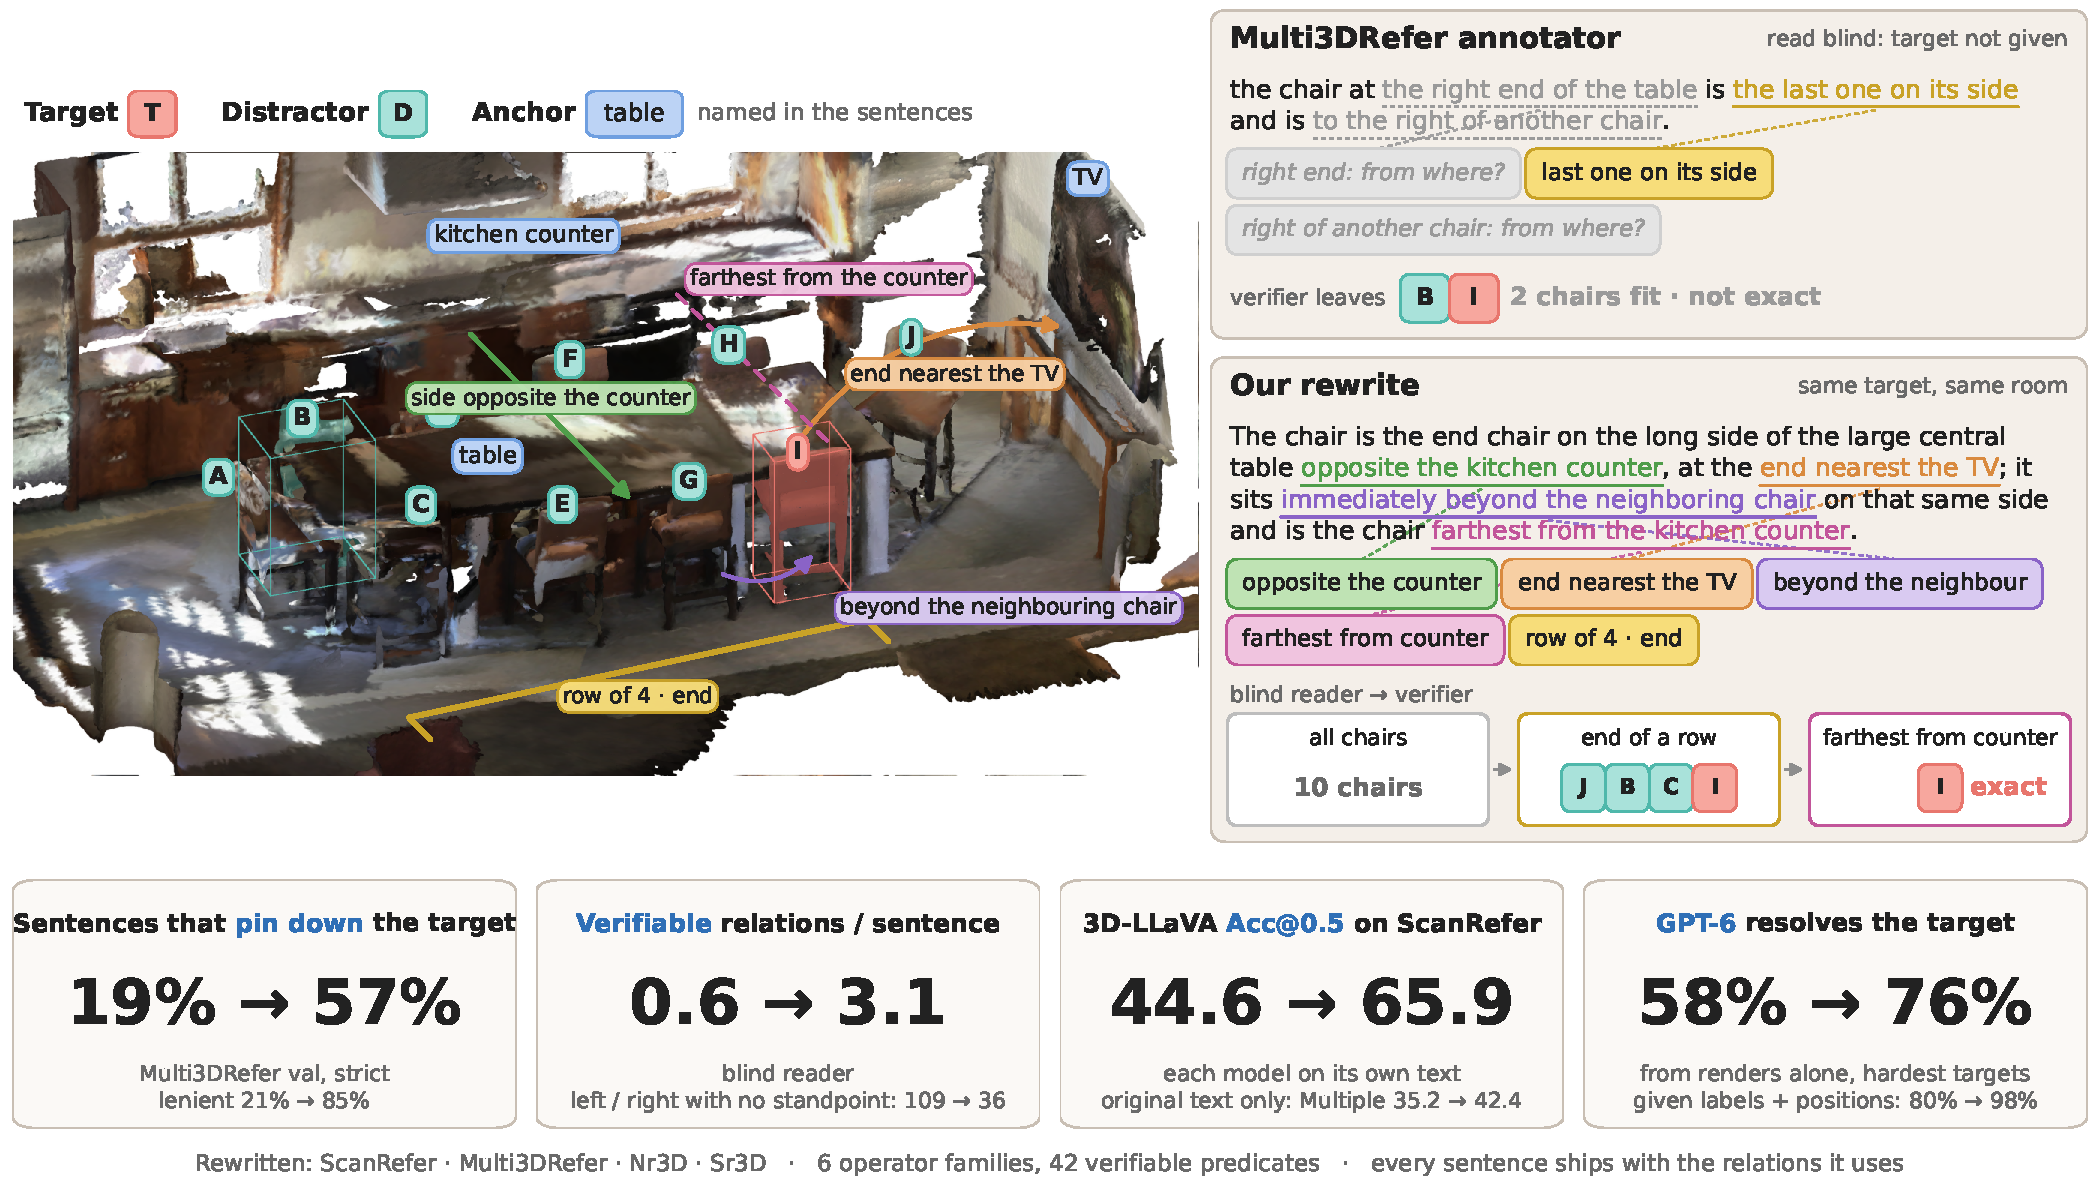
\includegraphics[width=\linewidth]{fig/teaser.pdf}
\captionsetup{hypcap=false}
\captionof{figure}{\textbf{A sentence that does not pin down its target, and the same target rewritten so that it does.}
A Multi3DRefer annotator describes chair~I in a ScanNet dining room (scene0011\_00).
Read blind---without being told the target---the only clause that binds to geometry is \emph{the last one on its side}, and two chairs satisfy it (B and I); \emph{right end} and \emph{right of} name no standpoint (grey).
Our rewrite uses anchors that exist in the room (the kitchen counter, the TV) and relations our operators computed and checked; each clause is coloured like its chip and like the relation drawn on the scene, and the same blind reader and verifier leave one chair.
Tags: target red, same-class candidates teal, anchors named by the sentences blue.
Bottom, left to right: how many sentences pin down their target; how many verifiable relations they carry; what 3D-LLaVA scores when each model is trained and tested on its own text (and, on the original text alone, on targets with same-class distractors); what GPT-6 resolves from the same renders.
\TODO{re-sync the four numbers with the final tables.}}
\captionsetup{hypcap=true}
\label{fig:\currfilebase}%
\end{strip}

% Source of truth for wording decisions: Seshat-Star/docs/PAPER_FRAMING.md §8f (user's 11-13 version, release sentence restored 11-14).
% 11-16 trims (user): reader's input list, "keeps the annotator's attributes and landmarks", "needs only a scene with instance labels" moved out of the
% abstract (they live in intro / method); "entirely" -> "almost entirely" (Unique moves 86.4 -> 87.4); "We release" -> "We will release".
% Terminology: "exact", not "unique" (clashes with ScanRefer's Unique/Multiple split).
% E5 numbers for the bracketed ceiling sentence (hard set, GPT-6, Acc@0.5): with full geometry (T1) 99% on rewrites / 80% on originals;
% from clean renderings alone (T3) 76% / 58%. Phrasing of that sentence still to be decided by the user.
\begin{abstract}
3D vision--language models learn where things are from referring expressions, and for years they have been trained and tested on sentences that, as we show, do not pin down the object they describe. A referring expression is correct only if it fits its target set exactly: a sentence in which every word is true can still be wrong when it fits one object too many, or one too few. To our knowledge, no published tool scores an arbitrary 3D referring expression on this criterion. We introduce one. A blind reader (a frontier model) translates the sentence into predicates over object ids; a deterministic verifier evaluates them on the point cloud; the sentence is exact when the objects satisfying every predicate are precisely the target set. By this measure, only about one in five human-written sentences in ScanRefer and Multi3DRefer is exact, and over half contain no checkable spatial relation. Moreover, 81\% of Multi3DRefer's multi-target sentences are ScanRefer sentences, written about one chair and labelled with four, so the same words carry two labels. Our pipeline, Seshat-Star, rewrites these expressions: a frontier model sees the rendered scene together with the relations a rendering hides (viewpoints, rows, stacks, room structure), computed by geometry; it decides what to say, and the scorer checks the result. Rewrites are exact three to four times as often and carry five times as many checkable relations. Trained on the rewrites, 3D-LLaVA gains 6 points of Acc@0.5 on the \textbf{original} ScanRefer validation set, almost entirely on targets with distractors. % 11-15: "it gets better at telling look-alikes apart, not at reading longer sentences" cut from the abstract (funnel: that reading lives in intro ¶6 and §6); restore if wanted.
On the hardest targets, a frontier model given every object's label and position resolves 98\% of them from the rewrites' spatial cues alone, against 80\% from the original sentences; from renderings alone, 76\% against 58\%. We will release the rewritten ScanRefer, Multi3DRefer, Nr3D and Sr3D, a distractor-heavy benchmark, and the scorer.
\end{abstract}

% Draft v3 (11-16): density lowered per the user -- the intro names things and gives headline numbers; how they work lives in the
% sections it points to. Details cut from v2 are parked as comments at the top of sec/3--6 so that nothing is lost.
% Layout unchanged from v2 (PAPER_FRAMING §1). Numbers in \TODO{} are placeholders or pending (human check, generation mode, further architectures).
% Human-check clause (P2), sentence level per the user (predicate-level E7-B, 82/104 = 79%, goes to the scorer section).
% 76% = E7 task A1, PRELIMINARY (3 annotators, still labelling; snapshot 11-16 late): scorer-strict-exact sentences, both arms, human picks exactly
% the target set 71/93, "can't tell" counted as a miss (user's call). Same data, NOT in the clause: sentences the scorer does not certify are
% still resolved 105/195 = 54%; humans resolve 52% of originals (75/144) and 70% of rewrites (101/144) -- these two are the human pair in the results paragraph (P6). The scorer is a conservative certificate, not a two-sided classifier -- see PAPER_FRAMING before freezing the wording.
% Replace the number when all annotators are in; keep it one clause.
% REFRESHED 11-16 21:33 CST snapshot (4 annotators, 536 judgements; Seshat-Star/analysis/_e7_snapshot.py): certified 129/173 = 75%
% (was 76), originals 127/271 = 47% (was 52), rewrites 185/265 = 70% (unchanged). Same numbers as tab:human in sec/4.
\section{Introduction}
\label{sec:intro}

In three years, 3D vision--language models have changed almost everything about how they look at a scene and almost nothing about what they read. They are trained and tested on the same handful of referring corpora, and what such a model learns about space is bounded by what that text says about space. The benchmarks have been generous: on most of their sentences a model can do well without reading much geometry (\cref{sec:related}). This is not a failing of the models; the text did not ask it of them. We set out to measure how much of that text actually does.

We call a referring expression \emph{exact} when it fits its target set and nothing else: no distractor left in, no target left out. No published tool scores a 3D referring expression on this criterion, to our knowledge, so we built one: a blind reader and a deterministic verifier (\cref{sec:scorer}). Of the sentences it certifies, human annotators resolve \TODO{75}\% to exactly the target set. On ScanRefer and Multi3DRefer it certifies \TODO{19}\% of human-written sentences, and finds nothing to check in \TODO{53--56}\% (\cref{sec:data}). An ambiguous sentence is not a neutral training example: it tells the model that these words mean several places at once, and the model's picture of the scene blurs to match.

Seshat-Star rewrites these sentences so that they are unambiguous, rich and verifiable---and still read as something a person would say. A division of labour makes this possible (\cref{sec:pipeline}). Geometry computes the relations that are hard to see in a rendering and easy to get wrong---which row and which seat in it, where to stand so that \emph{left} means something---and hands them to a frontier model as evidence. The model, not a template, decides which to use and how to say them: diversity comes from the free text, checkability from the computed relations. The geometric operators behind this evidence took most of the work, and everything else in the paper runs on them: the writer's evidence, the scorer's verifier and the benchmark.

One design choice follows from what we learnt about the model along the way. The scorer checks every rewrite, but its verdicts are never fed back into the writer: the model does whatever its evidence tells it to, so the only safe evidence is evidence that is true.
% 11-16: removed "And the improvement is not the base model's cleverness alone: the same writer, given better geometry, locks its target more
% often." -- the old-vs-new geometry control on judge600 (RESULTS §1.7) shows no difference (strict 56.0 vs 54.2, n.s.); the pilot's 19 -> 26 of 40
% was noise. To earn a sentence of this kind back, run the missing control: same writer, same 600 items, NO computed relations (render only).

We test what this does to models on 3D referring. The answer must be an object in the room, so a language prior cannot skip the scene as it can in question answering; and success on a sentence can be attributed to the class name or to the spatial cues, depending on how many same-class distractors the target has.

The rewrites are unambiguous: the scorer certifies \TODO{54}\% of them, up from \TODO{19}\%, and human annotators resolve \TODO{70}\%, up from \TODO{47}\%. They are rich: \TODO{3.2} checkable relations per sentence against \TODO{0.6}. They stay varied: \TODO{13}\% of the relations the writer uses lie beyond the verifier's vocabulary, without affecting how often a sentence is exact. And they need no original: given only a scene and a target, the pipeline writes sentences the scorer certifies just as often, on ScanNet and on scenes from 3RScan and Matterport3D (\cref{sec:data}). Trained on the rewrites rather than the originals, 3D-LLaVA moves from \TODO{44.6} to \TODO{50.7} Acc@0.5 on the original ScanRefer validation set, and from \TODO{35.2} to \TODO{42.4} on targets with same-class distractors: it is sharper at telling look-alikes apart, not at reading longer sentences. On the hardest targets, GPT-6 is \TODO{5 to 19} points more accurate reading the rewrites than reading the originals, across four levels of spatial information (\cref{sec:model}).

Our contributions are: (i) a set of geometric operators, 42 verifiable predicates, that compute the spatial relations a rendering hides; (ii) built on them, a scorer that measures whether a 3D referring expression is exact, and Seshat-Star, a rewriting pipeline in which geometry supplies the evidence, a frontier model writes, and the scorer checks; (iii) the rewritten ScanRefer, Multi3DRefer, Nr3D and Sr3D, every sentence carrying the relations it uses, a distractor-heavy benchmark, and a pipeline that writes for any scene with instance labels, with or without an original sentence; (iv) evidence that changing the training text alone makes a 3D grounding model sharper exactly where spatial cues are needed; (v) the ceiling: a frontier model's accuracy on the hardest targets under four levels of spatial information.

% Draft v1 (11-15). Organisation per Seshat-Star/docs/PAPER_FRAMING.md §1 ("三根轴" + corpora + models);
% facts and numbers from docs/RELATED_WORK.md and docs/CLAIMS.md §1–2. Third-party numbers are quoted from the cited papers;
% items marked TODO in main.bib still need author/title verification.
\section{Related Work}
\label{sec:related}

\paragraph{Generated referring language for 3D scenes.}
Most 3D referring text that people did not write is produced by one recipe: a scene graph or a program holds the geometry, a template or a constraint sampler turns it into a specification that singles out the target, and a language model paraphrases the result. Sr3D~\cite{referit3d} fills templates over relations that hold for the target and for no other object of its class; SceneVerse~\cite{sceneverse} and 3D-GRAND~\cite{3dgrand} have GPT write from the graph; Disc3D~\cite{disc3d} enumerates subsets of appearance, size and relation modifiers until their intersection is exactly the object; CLEVR-3D-DeRef~\cite{clevr3dderef} executes functional programs~\cite{clevrrefplus} on synthetic scenes; and ViGiL3D++~\cite{vigil3d,vigil3dpp}, the closest work to ours, samples constraints from a graph of real scans---including directions from a sampled standpoint and ordinals along a row---until the solution set is the target. These pipelines differ in detail and agree on three things.
\emph{Uniqueness is guaranteed before the text exists}, on the graph or in the program, and the last step is a free-form rewrite after which nothing returns to the geometry: CLEVR-3D-DeRef scores its paraphrases by how many attribute and relation words they share with the template, not by executing them again, and ViGiL3D++ passes its sentences through a second model to repair grammar and ambiguity.
\emph{The language model is a paraphraser.} What the sentence says is fixed upstream and the model changes the words; Disc3D's vision model is asked whether one rule-given relation holds between two boxed objects in a single frame and, if it says no, chooses a replacement from a closed list; viewpoint words---\emph{front}, \emph{behind}, \emph{left}, \emph{right}---are forbidden outright, and its spatially anchored sentences keep a single distinctive relation.
\emph{Nobody measures the finished sentence.} Where the authors did, the cost of the first two choices shows. ViGiL3D++'s own human check finds that single-target sentences whose target has same-class distractors are valid 43.1\% of the time, although each relation in its graph is 89.7\% accurate: composition, missing graph nodes and paraphrase drift are paid for at the sentence and never charged to it. 3D-GRAND reports 91.8\% grounding correctness from crowd-workers asked whether a phrase refers to the boxed object; the same corpus scores 38.3\% when the standard adds \emph{and nothing else fits}~\cite{vigil3dpp}. Disc3D's revision of its test set covered the comparative sentences and left the spatially anchored ones unchecked. Correct but not exact is the normal case in generated text, as we will show it is in human text (\cref{sec:data}).

We differ on all three counts. We keep the sentence a person wrote and let a frontier model decide what to add, given computed facts it could not see; we verify \emph{after} the text, reading the final sentence back into predicates and executing them on the scene; and every sentence receives a score, which is how we can report a number for ScanRefer itself---something no construction-time guarantee can do. Keeping the human sentence also avoids a cost that generating from scratch pays on human benchmarks: a model trained only on ViGiL3D++ scores below the same model trained only on human-written data on ScanRefer and Multi3DRefer (45.5 against 53.4, 23.1 against 33.5), and recovers only when the human data is mixed back in~\cite{vigil3dpp}. Beacon3D~\cite{beacon3d} is complementary rather than competing: it documents, by a human study, that the text of existing grounding benchmarks is ambiguous, and re-annotates thirty scenes to test on; we measure the ambiguity geometrically and repair the training corpora at scale.

\paragraph{The corpora.}
ScanRefer~\cite{scanrefer} attaches one description to one object; Nr3D~\cite{referit3d} does the same through a reference game played among same-class distractors; Multi3DRefer~\cite{multi3drefer} extends ScanRefer to zero, one or several targets, and its convention is that a description matching several objects is labelled with all of them. Under that convention a plural reference (\emph{the two pillows}) and an under-specified one (\emph{a pillow}, with two on the couch) receive the same kind of label. The two corpora share words and disagree about what they mean: 81\% of Multi3DRefer's multi-target validation sentences are paraphrases of ScanRefer sentences about the same scene,\footnote{Word Jaccard $\ge 0.5$ with the ScanRefer target among the Multi3DRefer targets; 529 pairs are at $\ge 0.7$ and 39 are near-verbatim.} labelled with one chair in one corpus and with four in the other; conversely, 21\% of the sentences in ScanRefer's \emph{Multiple} validation split were judged by Multi3DRefer's annotators to fit at least two objects, where ScanRefer accepts one. Neither corpus breaks its own rules; the sentence is under-specified and each convention resolves it differently. Nanri et al.~\cite{nanri2026viewpoint} make the related observation that neither corpus handles observer-dependent relations such as \emph{left} and \emph{right}, and build a synthetic corpus in which the viewpoint is supplied to the model as a camera pose; we write the standpoint into the sentence instead, so that no input channel is added (\cref{sec:pipeline}).

\paragraph{Models, and where geometry enters.}
Recent 3D grounding models admit geometry in four different ways. Chat-Scene~\cite{chatscene} represents each object by an identifier token carrying Uni3D and DINOv2 features and no coordinates; QuatRoPE~\cite{quatrope} keeps that recipe and adds object centres to attention through a quaternion rotary encoding; Video-3D-LLM~\cite{video3dllm} and 3DRS~\cite{3drs} add an encoding of each patch's world coordinates to the visual features, the most explicit of the four; 3D-LLaVA~\cite{3dllava} uses sparse U-Net shape features and an isotropic distance bias, with no explicit coordinates and no orientation. The protocols differ (box against mask IoU), so the scores cannot be subtracted, but they sit in one band, 55 to 64 Acc@0.25 on ScanRefer, and adding a coordinate channel to Chat-Scene moved its score by 2.3 points. Third parties have reached the same conclusion from the other side: 3D-LLaVA, evaluated zero-shot on referring expressions that contain nothing but a direction, scores a mean IoU of 0.08~\cite{nanri2026viewpoint}; Beacon3D~\cite{beacon3d} finds that a language model fine-tuned on SQA3D~\cite{sqa3d} without seeing the scene scores unexpectedly well, and that paraphrasing a referring expression moves grounding scores. Our reading is not that these models cannot use geometry but that the text they are scored on seldom requires it. \cref{sec:model} asks what happens when it does: with the architecture of 3D-LLaVA untouched, changing only what the training text says about space moves its Acc@0.5 on the same validation set by six points\TODO{; further architectures pending}. Finally, GR3D~\cite{gr3d_zillow} shows that a frontier model answers spatial questions better when given geometric text about the scene, and that the gain disappears when that text is not bound to identifiers marked in the image---the same identifier-bound design that our writer and reader rely on (\cref{sec:pipeline,sec:scorer}).

% Claims and numbers for this section: Seshat-Star/docs/CLAIMS.md; narrative: docs/PAPER_FRAMING.md
% --- Parked from intro v2 (11-16): say these here, in new words, not in the intro ---
% * What geometry computes: which end of the room, which row and which seat in it, what rests on what, where to stand so that left means something.
% * Operators: six families, 42 predicates; each revised against human inspection of real rooms until what it reported matched what a person sees.
% * The model keeps the annotator's own attributes and landmarks (also cut from the abstract).
% * The writer names relations in some 2,400 ways, the verifier needs to recognise 42; sentences read as descriptions, not filled templates.
% * An earlier version (a menu of relations + a smaller model to phrase them) produced little worth keeping; the same frontier writer given
%   better geometry locks its target more often (19 -> 26 of 40, pilot; number still to be confirmed).
% * Runs on any real scene with instance masks, with or without an original sentence (was contribution (iii); generation-mode number pending).
\section{The Seshat-Star pipeline}
\label{sec:pipeline}

\TODO{to be drafted}

% Claims and numbers for this section: Seshat-Star/docs/CLAIMS.md §4; RESULTS.md §1.4, §3.4, §4; narrative: docs/PAPER_FRAMING.md
% v1 drafted 11-16.  Number provenance (check before freeze):
% * Blind vs aware reader 16.5 -> 17.5 on originals, n = 200 pairs: RESULTS §1.4 (10-21 run, older verifier).
% * Wrong-target probe 2 of 15: RESULTS §3.4 (scene0549_00_ann39 is the inspected case). n is small; do not quote an interval.
% * Human check (tab:human, and 75 / 79 / 12 / 51 in the text): E7-A1 SNAPSHOT, analysis/_e7_snapshot.py.  12% / 51% = scorer
%   certifies 23 / 101 of the 200 A1 items (a1_items.jsonl, field `ours`).  79% = P(second annotator resolves | first resolves) = 146/186.
% * Predicate cards (E7-B SNAPSHOT, 218 judgements): three self-defined families 114/146 = 78%; stacks 53/61 = 87%; rows 26/35;
%   faces 35/50; control next_to 37/44 = 84%; near misses 35/53 = 66%; clear negatives 36/40 = 90%.
% * GPT-6 98 / 96 / 90 (n = 536 / 248 / 349): CLAIMS §4 "E5-fail", hard/e5_fail/REPORT.md.  T2 = labels + positions (oracle perception).
% * Surface-gap correction, 9.5% of closest / farthest claims: RESULTS §4.5 (11-12).
% * Writer's own relations vs the reader's, 15--25 points: RESULTS §1.6 (generation mode); quoted in sec/5.
% Parked for the supplement: q-sensitivity (3.5 / 7.2 / 14.5% at q = 0.05 / 0.10 / 0.20), text-channel loss by relation family,
% unbound-reason distribution, verifier revision history, per-family human table.
\section{Scoring exactness}
\label{sec:scorer}

\paragraph{Definition.}
Let $T$ be the target set of a sentence, $C \supseteq T$ its candidates and $D = C \setminus T$ its distractors (\cref{sec:pipeline}).
The reader turns the sentence into predicates $p_1,\dots,p_K$ over object ids; the verifier evaluates each on the scene and returns $\hat{E}_k \subseteq C$, the candidates that satisfy it.
The sentence is \emph{certified} when
\begin{equation}
  K \ge 1 \quad\text{and}\quad \bigcap_{k=1}^{K} \hat{E}_k = T .
  \label{eq:exact}
\end{equation}
It can fail in two ways: a distractor survives every predicate, or one predicate excludes a target.
A sentence that coordinates groups (\emph{the two by the window and the one at the door}) is read in parts; predicates conjoin within a part and the parts are united (\supp{supp:parts}).
The condition $K \ge 1$ is deliberate.
A sentence that offers nothing to check is not certified, even when its target is the only object of its class and the class name would do: we score what the sentence says about space.

\paragraph{The reader is blind.}
The reader is GPT-5.5 with the sentence and the room's instance list.
It does not see the target, the candidates, our evidence or the relations the writer reported, and for every clause it cannot bind to object ids it must give the reason: no viewpoint, ambiguous anchor, object not in the list, not spatial.
We keep it blind because a reader that knows the answer reads toward it.
Given a \emph{wrong} target on purpose, it certified that object in 2 of 15 trials, in one of them by silently dropping the two clauses that excluded it.
Blindness costs little: in an earlier run of 200 pairs, telling the reader the true target raised the rate of the original sentences by one point.

\paragraph{The verifier contains no model.}
It evaluates 42 predicates on the instance table and the points: proximity (\emph{next to}, \emph{closest to}, \emph{touching}, \emph{between}), support and vertical order, places in the room (wall, corner, centre), directions from a stated standpoint, rows and positions in them, and the faces and ends of large furniture (\supp{supp:vocab}).
The same input always gives the same verdict.
With the operators that produce the writer's evidence it shares only a few measuring primitives---surface gap, support, collinearity, row decomposition; above these, neither calls the other.
An error in a primitive therefore shows on both sides, while an error above them stays on one, so the verifier's output is audited on its own, below.

\paragraph{Strict and lenient.}
A predicate the reader extracts can be false of the target itself.
The \emph{strict} score intersects it like any other, and the sentence fails; the \emph{lenient} score skips it.
The two differ in this rule and nothing else.
A skipped predicate may be the writer's mistake, the reader's over-translation (\emph{along the wall} read as \emph{against the wall}) or the verifier's rigidity (a wall test in a room that is not a rectangle).
We cannot yet separate the three, so we report both and take the strict score as the measurement.

\paragraph{A lower bound.}
Write $E_k$ for the candidates that truly satisfy $p_k$.

\noindent\textbf{Proposition 1.} \emph{Suppose that for every $k$ the verifier has no false positive on a target, $\hat{E}_k \cap T \subseteq E_k$, and no false negative on a distractor, $E_k \cap D \subseteq \hat{E}_k$. Then $\bigcap_k \hat{E}_k = T$ implies $\bigcap_k E_k = T$.}

\noindent Under these assumptions every strictly certified sentence is truly exact, and the certified rate bounds the true rate from below (proof and sensitivity analysis in \supp{supp:proof}).
The assumptions concern opposite errors on complementary sets, so no overall accuracy of the verifier implies either of them.
They will not hold perfectly, and the proposition takes the predicates as given; it says nothing about what the reader failed to recover.
We therefore also measure the scorer against people.

\paragraph{Against people.}
Annotators saw a scene as an interactive point cloud with the candidates lettered at random, and one sentence, without knowing whether it was an original or a rewrite; they selected every object the sentence fits (\cref{tab:human}).
Three things follow.
The scorer is conservative: people resolve \TODO{47}\% of the originals and \TODO{70}\% of the rewrites, where the scorer certifies \TODO{12}\% and \TODO{51}\% of the same items.
A sentence it does not certify is one whose uniqueness cannot be established from its spatial relations; a person may still find the object by its colour or by common sense, which the verifier does not see.
A certificate is worth about a second opinion: annotators resolve \TODO{75}\% of certified sentences, and when one annotator resolves a sentence a second does so \TODO{79}\% of the time.
And people and scorer order the sentences alike: human success falls as same-class objects multiply, and falls furthest for the originals.

We also checked the verifier predicate by predicate, on the structures we define ourselves: rows, furniture faces and stacks.
Annotators judged single statements with the objects marked, half of them made false by pointing at an object the verifier excludes.
They agree with the verifier on \TODO{78}\% of the statements they could decide (\TODO{84}\% for plain adjacency, the control), and disagreement concentrates on near misses: \TODO{66}\% agreement there against \TODO{90}\% on clear cases.
The verifier has been wrong before in exactly this way.
Until a human reader caught it, it measured gaps between boxes instead of surfaces, which changed the winner in 9.5\% of \emph{closest} and \emph{farthest} claims; the certified rates in \cref{sec:data,sec:model} all follow the correction (\supp{supp:ruler}).

A reading by a different machine agrees in order.
On distractor-heavy targets, GPT-6 reads the rewrite with every object's label and position at hand and nothing from the scorer; it resolves 98\% of the strictly certified sentences, 96\% of those certified only leniently and 90\% of the rest (\cref{sec:model}).
A rejection means \emph{not certifiable from the sentence}, not \emph{unsolvable}.
% Source: /data/sujie/horus/_rerun/e7 (task A1), computed by Seshat-Star/analysis/_e7_snapshot.py.
% SNAPSHOT 11-16 21:33 CST: 536 judgements, 4 annotators, 380 of 400 (item, arm) units; annotation still running.
%   all:           orig 127/271 = 46.9   rewrite 185/265 = 69.8
%   certified:     orig  22/32  = 68.8   rewrite 107/141 = 75.9   (both arms 129/173 = 74.6)
%   not certified: orig 105/239 = 43.9   rewrite  78/124 = 62.9   (both arms 183/363 = 50.4)
%   same-class objects <=2: 52/72, 64/68;  3-5: 43/70, 52/67;  6-9: 23/65, 38/69;  >=10: 9/64, 31/61
% "cannot tell" / "none fits" count as a miss (user, 11-16).  Re-run the script and refresh when annotation closes.
\begin{table}[t]
\centering
\small
\caption{\textbf{People against the scorer.} Share of judgements (\%) in which an annotator selects exactly the target set, on 200 validation items shown as the original or as the rewrite; ``cannot tell'' counts as a miss. \TODO{Snapshot: 536 judgements by four annotators; refresh when annotation closes.}}
\label{tab:human}
\begin{tabular}{@{}lcc@{}}
\toprule
Annotator resolves the sentence & Original & Rewrite \\
\midrule
All items & 47 & 70 \\
\addlinespace
Scorer certifies it (strict score) & 69 & 76 \\
Scorer does not & 44 & 63 \\
\addlinespace
Same-class objects: at most 2 & 72 & 94 \\
\quad 3--5 & 61 & 78 \\
\quad 6--9 & 35 & 55 \\
\quad 10 or more & 14 & 51 \\
\bottomrule
\end{tabular}
\end{table}


% Claims and numbers for this section: Seshat-Star/docs/CLAIMS.md; narrative: docs/PAPER_FRAMING.md
\section{What the rewrites contain}
\label{sec:data}

\TODO{to be drafted}

% Claims and numbers for this section: Seshat-Star/docs/CLAIMS.md; narrative: docs/PAPER_FRAMING.md
% --- Parked from intro v2 (11-16): say these here, in new words, not in the intro ---
% * 3D-LLaVA on the original ScanRefer val: overall Acc@0.5 44.6 -> 50.7; with same-class distractors 35.2 -> 42.4; targets without distractors do not move (the control).
% * For scale: adding a geometry channel with the training text unchanged moved ScanRefer accuracy by about two points (other protocol; see related work -- do not subtract).
% * E5: GPT-6 under four levels of information, from the sentence plus a list of class names up to every object's position and the relations
%   computed between them; rewrites stripped of their attribute words; they lead at every level, by 5 to 19 points.
\section{What models learn from them}
\label{sec:model}

\TODO{to be drafted}

% Claims and numbers for this section: Seshat-Star/docs/CLAIMS.md; narrative: docs/PAPER_FRAMING.md
\section{Discussion and Limitations}
\label{sec:discussion}

\TODO{to be drafted}

{
    \small
    \bibliographystyle{ieeenat_fullname}
    \bibliography{main}
}

% WARNING: do not forget to delete the supplementary pages from your submission
% \clearpage
\setcounter{page}{1}
\maketitlesupplementary

% --- To write (user, 11-16): be honest about the base model and about what failed ---
% * The writer is a frontier model (GPT-5.5, high effort); its capability is part of the result. The intro says "not the base model's
%   cleverness alone" -- that sentence was REMOVED 11-16 (old-vs-new geometry shows no difference, RESULTS §1.7). The control still missing is same writer WITHOUT computed relations.
% * Early attempts that failed, if the main text has no room: the menu-of-relations pipeline with a smaller model to phrase them (little
%   worth keeping), and whatever else PAPER_FRAMING / RESULTS record as abandoned. One short appendix section.
\section*{Summary of additional results}
\TODO{One table, three lines: which architectures, how many seeds, whether the direction agrees. Written last.}


\end{document}
